% !TeX root = RJwrapper.tex
\def\arraystretch{2.5}
\title{\emph{countfitteR}: Count Data Analysis for Precision Medicine}
\author{by Jaros\l{}aw Chilimoniuk, Alicja Gosiewska, Stefan R\"{o}diger and Micha\l{} Burdukiewicz}

\maketitle

\abstract{
\emph{countfitteR} is a package for the analysis of count data and selection of the most optimal distribution. It provides means to detect alterations in statistical dispersion through fitting data to four available distributions: Poisson, Negative Binomial (NB), Zero-Inflated Poisson and Zero-Inflated Negative. Our framework offers means to address bias in count data, including excessive zeros as well as over- and underdispersed counts. As a case study, we present the analysis of DNA damage using the phosphorylated histone variant H2AX ($\gamma$H2AX), an important biomarker in precision medicine. Our package comes with a Shiny web server dedicated to data scientists less fluent in \textbf{R}. \\
\emph{countfitteR} streamlines the 

}

\section{Introduction}
\subsection{Count data in precision medicine}

Count data represent the number of occurrences per event (for example a number of passengers per car) as non-negative integer values. It is one of the common data types with examples found in multiple fields. Some of them, for example, transportation safety, adverse drug events (ADEs), laboratory tests, require a more rigorous analysis, because failure can lead to serious consequences. In particular, in precision medicine counts of double strand breaks (DSBs) are an important biomarker of physiological and pathological cellular processes during radiation treatment~\citep{LomaxBiologicalconsequencesradiationinduced2013}. Therefore, they serve to assess patients well-being and their response to the therapy~\citep{reddig_dna_2018}.

%Sophisticated statistical bioinformatics procedures are an essential element of precision medicine \citep{deigner_precision_2018}. 
The role of DSBs in precision medicine is not limited to the quantification of DNA damage introduced by radiation, but also cellular processes or toxic agents used during chemotherapy. In general, quantification of DSBs allows researchers and clinicians to measure the extent of collateral DNA damage during the treatment~\citep{eberlein_calibration_2015, ivashkevich_use_2012}. Precise quantitative information could help to personalize treatment, e.g., the dosage of drugs to individual patients, and thus improve patient outcomes \citep{redon_recent_2011}. %It was shown that genetic polymorphisms of the H2AX gene can be associated with the level of DNA damage \citep{sun_genetic_2015}. Such specific information could be taken into account when modelling the cellular response to treatment.

We adopted a system that facilitates the digital enumeration of DSBs via the phosphorylated histone variant H2AX ($\gamma H2AX$)~\citep{rodiger_quantification_2018, ruhe_effect_2018}, which gather at DSBs sites creating a so-called focus~\citep{nikolova_h2ax_2014}. Thus, foci counting (counting number of foci per cell) is considered an efficient way to detect DSBs. Although these biomarkers play a crucial role in diagnostics, their levels vary not only between patients but also between replicates (CITATION NEEDED).

%In addition, associated biomarkers such as the p53-binding protein 1 (53BP1) may also be detected during the screening.

The variability can be decreased using a dedicated software~\citep{LapytskoFoCosimplerobust2015}, but still many factors may affect the foci counting procedure. As the number of DSBs may be one of the key factors deciding about the future therapy, we need a precise and unbiased method to estimate the real number of counted foci.  

%The Poisson distribution is presumably most commonly used when dealing with count data. However, in the context of DSBs, real foci data often do not satisfy constraints implied by this distribution. This suggests that another probability distribution for positive integers may describe a data set more accurately. Therefore, an identification of the probability distribution of $\gamma H2AX$ foci and associated biomarkers is vital for the precise estimation of the mean number of foci per cell and its confidence intervals.

\subsection{Over- and underdispersion}

To address this need, we propose a novel framework that allows in-depth investigation of counts. Although our methodology uses well-known and already published techniques, we hope that our tool will be more approachable to a wider audience of data analysts.

Our tool focuses on the unbiased estimation of mean and variance, two first moments of probability distributions. In the case of count data, the mean is the average number of occurrences per event. The variance can be seen as the fluctuation of occurrences per events, for example the high variance implies a large number of extremely high or low counts. The Poisson distribution, commonly used in the analysis of count data, assumes that mean and variance are equal. However, it is often the case that variance is larger than mean (overdispersion) or lower than mean (underdispersion)~\citep{Coxremarksoverdispersion1983, morina_generalized_2015_2}.

To model over- or underdispersed data, we require a different probability distribution. The negative binomial (NB) best describes situation when the variance is affected by the increased presence of extremely high or low counts. Despite the fact that the NB distribution is used primarily for counting the number of failures before a predetermined number of successes occurs, it can be also alternatively parametrized to describe count data with non-equal variance and mean. One of the important properties of the NB distribution is that the maximum likelihood (ML) estimator of its mean ($\hat{\mu}$) (e.g., the mean number of occurences per event) is equal to the arithmetic mean of counts in a data set.

The second cause of overdispersion considered by us is zero-inflation, an excessive number of zeros in a data set. We distinguish two causes for zero-inflation. Either zeros occur naturally or false zeros are introduced by an unknown factor (e.g., foci not detected by the system). To describe zero-inflation we use the Zero-Inflated Poisson (ZIP) and the Zero-Inflated Negative Binomial (ZINB) distributions. The former is used to depict Poisson-distributed data, where overdispersion is caused by the excessive zeros. The latter for data where overdispersion arises from both increased variability of counts and zero-inflation. It is important to note, that in case of zero-inflated distributions, the mean number of counts $\lambda$ is not equal to the average number of foci per cell ($\mu$). To describe their relationship, we need to introduce another parameter, r, which is equal to the fraction of counts faulty turned to zeros. Using the introduced notation: $\lambda = \frac{\mu}{1 - r}$. Henceforth, if we do not correctly identify zero-inflation, we underestimate the real number of foci per cell.

Overdispersed distributions in most cases have variance larger than the Poisson-distributed counts with the same average number of foci per cell ($\lambda$). In consequence, the confidence intervals are wider than in the case of the Poisson distribution. It directly affects the conclusion drawn from a data analysis. Because bigger change of the mean number of foci is required, to support the significance of the impact of the treatment. 

Since overdispersion has serve impact on a data analysis, we created \emph{countfitteR} for determination of the count data distribution. Our software fits count data to four distributions, that describe counts: Poisson, NB, ZIP and ZINB. Although statistical tests designed for detecting overdispersion exist, they work properly only in a specific range of values. These tests only indicate if the data is overdispersed, but do not point the suitable probability distribution. Therefore, \emph{countfitteR} selects the most appropriate model using the Bayesian Information Criterion (BIC). The analysis is coupled with an estimation of parameters in the distribution of choice and their confidence intervals.  

\subsection{Applications}

In the following we will focus on counting data where there is a need in the field of laboratory medicine. In addition, there are other areas of application for counting data. Examples are transportation research \citep{narayanamoorthy_accommodating_2013}, meteorology, \citep{brijs_studying_2008} and clinical research \citep{keene_analysis_2007}.


\section{Models}

In \emph{countfitteR} we have implemented 3 variants of the distribution equations. They are selected according to the specifications of the dataset. %Examples are given below.

Parameters:
\begin{itemize}
\item $\lambda$ - Poisson parameter (average number of foci per cell). 
\item $r$ - zero inflation (fraction of cells treated by system as having no foci regardless of their real state).
\item $\theta$ - dispersion parameter.
\end{itemize}

\subsection{Variant 1}

Usually the NB distribution is parameterized using $\mu$ and $\theta$, but to make comparison clearer, we use $\lambda$ instead of $\mu$. In this parameterization, NB and ZINB are treated as the mixture of Poisson and Gamma ($\Gamma$) distributions.  

\begin{center}
\begin{tabular}{ |c|c| } 
\hline
\bfseries Distribution name & \bfseries pmf \\
\hline
Poisson & $P\{X = k\} = \frac{\lambda^k \exp^{-\lambda}}{k!} $ \\
\hline
Zero-inflated Poisson & $P\{X = k\} = \begin{cases} r + ( 1- r) \exp^{-\lambda},\text{if } k = 0\\ r \frac{\lambda^k \exp^{-\lambda}}{k!},\text{if } k = 1, 2, \ldots \end{cases} $ \\
\hline
Negative Binomial & $P\{X = k\} = \frac{\Gamma (\theta + k)}{\Gamma(\theta) k!}  \left( \frac{\theta}{\theta + \lambda} \right)^\theta \left( \frac{\lambda}{\theta + \lambda} \right)^k$ \\
\hline
Zero-inflated Negative Binomial & $P\{X = k\} = \begin{cases}r + (1 - r) \left( \frac{\theta}{\theta + \lambda} \right)^\theta,\text{if } k = 0\\(1 - r) \frac{\Gamma (\theta + k)}{\Gamma(\theta) k!}  \left( \frac{\theta}{\theta + \lambda} \right)^\theta \left( \frac{\lambda}{\theta + \lambda} \right) ^k,\text{if } k = 1, 2, \ldots\end{cases}$ \\
\hline
\end{tabular}
\end{center}

\subsection{Variant 2}

Poisson and Negative Binomial distributions have the same expected value. In case of ZIP and ZINB, the expected value is smaller than the real average number of foci per cell.

% ###################################### change to real average number or leave of foci per cell ?

\begin{center}
\begin{tabular}{ |c|c| } 
\hline
\bfseries Distribution name & \bfseries Expected value \\
\hline
Poisson & $E(X) = \lambda $ \\
\hline
ZIP & $E(X) = (1 - r) \lambda $ \\
\hline
NB & $E(X) = \lambda $ \\
\hline
ZINB & $E(X) = (1 - r)  \lambda $  \\
\hline
\end{tabular}
\end{center}parameterization

\subsection{Variant 3}

Depending on the value of $r$ the variance of ZIP and ZINB may be smaller or bigger than the variance of Poisson distribution. In case of the NB distribution, the variance is always bigger than for the Poisson distribution, although the difference becomes negligible, when the $\theta$ is much bigger than $\lambda^2$.

\begin{center}
\begin{tabular}{ |c|c| } 
\hline
\bfseries Distribution name & \bfseries Variance \\
\hline
Poisson & $\textrm{var}(X) = \lambda $ \\
\hline
ZIP & $\textrm{var}(X) = \lambda (1 - r)(1 + \lambda r)$ \\
\hline
NB & $\textrm{var}(X) = \lambda + \frac{\lambda^2}{\theta} $ \\
\hline
ZINB & $\textrm{var}(X) = (1 - r) \lambda \left( 1 + r\lambda  + \frac{\lambda}{\theta} \right)$ \\
\hline
\end{tabular}
\end{center}


\section{\emph{countfitteR package}}

%\section{Describe briefly main functions}

\emph{countfitteR} provides clinical scientists with a simple interface for the analysis of count data regardless of their biostatistical knowledge about the nature of the distribution. The framework covers two most common situations. In the first approach, each count is separately fitted to all above mentioned distributions. This is preferable for situations, where counts come from various sources. The second approach relies on fitting globally all counts to a distribution. Such model is appropriate among others for technical replicates.
Our software is open source and accessible also from the command-line level. It is suitable for integration into other analysis pipelines dealing with count data. Therefore, we anticipate that our finding will have a broader use. 
The web server is accessible under: 
\url{update me}
% #############################################################################3 add web server url

\section{Data sets}
In the present study we used count data from an image based study of $\gamma H2AX$ foci. The data was generated from human peripheral blood mononuclear cells (PBMCs). PBMCs were treated with the topoisomerase inhibitor etoposide to induce $\gamma H2AX$ foci. Analysis of such foci data is a common task both in life sciences and in diagnostics applications. \emph{countfitteR} was initially developed for modeling count data from the AKLIDES system, but it may be used for foci data from other systems.
The data were prepared as described in \citep{rodiger_quantification_2018}. The Comprehensive R Archive Network (CRAN), which archives R packages, has a recommended size limit of five megabytes (MB) \citep{anderson_hosting_2017}. Therefore, the following data sets are include only.

\newpage

{\bfseries
\begin{example}
>foci_count[1:15, 1:5]
\end{example}
}

{\scriptsize
\begin{example} 
   L3_AF_DMSO_B_10_FITC L3_AF_DMSO_B_10_APC L3_AF_100_ETP_11_FITC L3_AF_100_ETP_11_APC L3_AF_100_ETP_12_FITC
1                     0                   0                     0                    0                     0
2                     0                   0                     0                    1                    19
3                     0                   0                     0                    0                     0
4                     0                   0                     1                    0                    12
5                     0                   0                     0                    0                     4
6                     0                   0                    13                    0                     1
7                     0                   0                     0                    0                     0
8                     0                   0                     0                    0                     3
9                     0                   0                     0                    0                     8
10                    0                   0                    12                    0                     0
11                    0                   0                     5                    0                     0
12                    0                   0                    21                    0                     0
13                    0                   0                     0                    0                     0
14                    0                   0                     0                    0                     0
15                    0                   0                     0                    0                    11
\end{example}
}

The data of human PBMCs was already published. It was used to show that freezing of PBMCs did not influence the amount of $\gamma H2AX$ foci formation. However, the results of this experiment where statistically analysed using GraphPad Prism.
% When the publication is out, we can add it to this paper otherwise we have to say that the data will be published.


\section{Shiny GUI} %Graphical User Interface

Our application is available as a web server that may be used in an analysis of any kind count data, not only $\gamma H2AX$ and 53BP1. It is accompanied by an in-depth manual depicting the implemented framework and a rationale behind it. The guide covers both theoretical fundamentals and usage of \emph{countfitteR}, from a data import to a report generation.

In case the web server is offline or connection to the Internet is restricted, access to the package’s capabilities is done by using the command in the R console. It initiates a graphical user interface (GUI), which starts shiny server on a local pc, it runs as long as the window is open. This mode can be named "serverless mode", as it does not require external server to run.

%\begin{figure}[htbp]
%  \centering
%  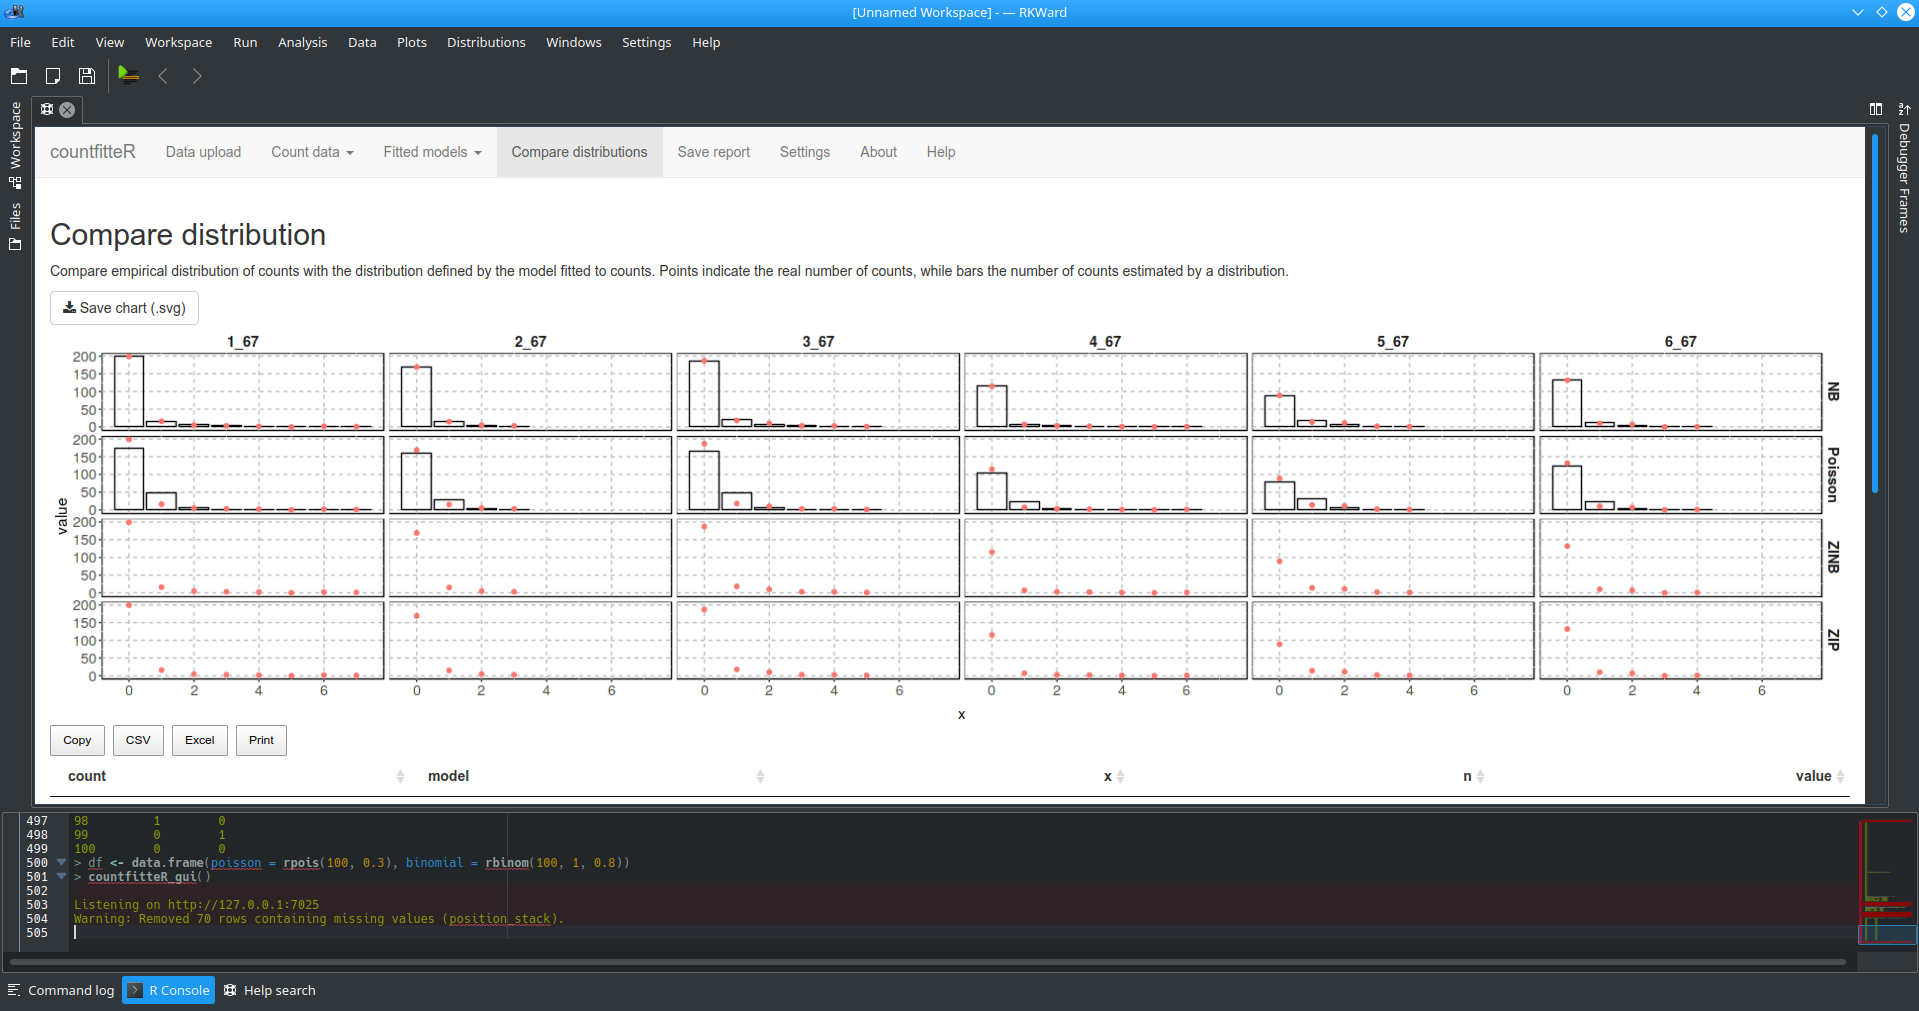
\includegraphics[width=0.99\columnwidth]{fig_gui}
%  \caption{\emph{countfitteR\_gui()} function running in the \emph{RKWard} GUI/IDE (v. 0.7.0z+0.7.1+devel1) on Kubuntu 18.04. \citep{rodiger_rkward:_2012}.}
%  \label{fig_gui}
%\end{figure}

In \textit{Data upload} tab the csv file with count data can be uploaded (Figure \ref{cf_main}). But before that one of csv separators types must be selected to properly load file. If the data file does not have a header the box should be unchecked. If no file will be uploaded, example file will be loaded.

%\begin{figure}[htbp]
%  \centering
%  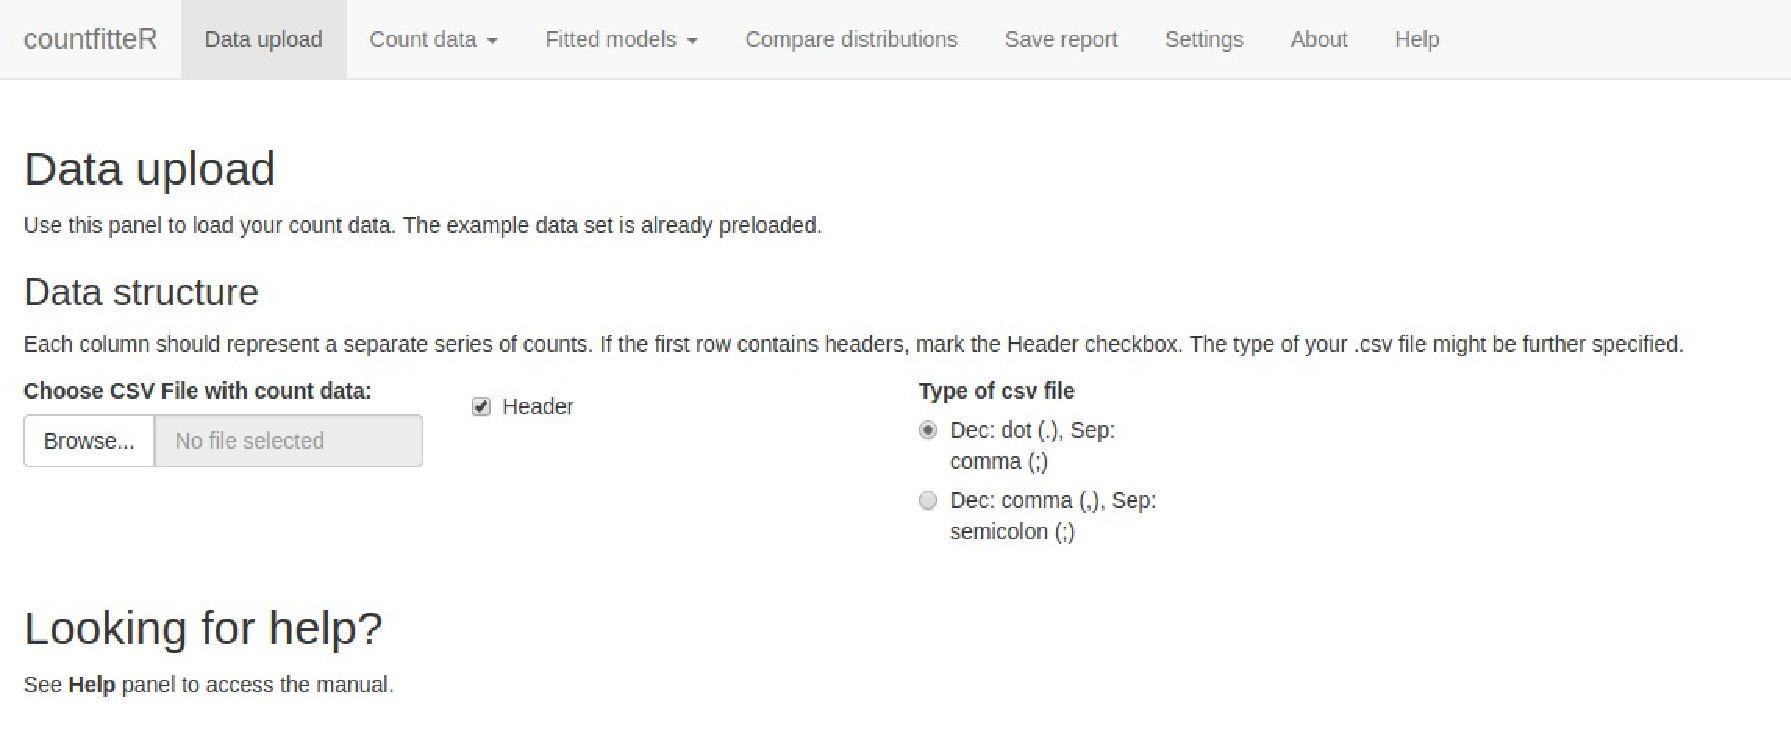
\includegraphics[width=0.99\columnwidth]{fig/cf_main.pdf}
%  \caption{Starting page of the \emph{countfitteR} shiny GUI, where user can upload their data.}
%    \label{cf_main}
%\end{figure}

In \textit{Count data} tab there are 3 submenus. \textit{Edit input data}, where the loaded data can be reviewed and also modified (addition and removal of values and rows) if needed
% (Figure \ref{cf_cd1})
. However, changes will not be tracked and reported in the summary. \textit{Summary} summarizes statistics of data in table (Figure \ref{cf_cd2}). In \textit{Distribution} menu the distribution of counts are displayed in form of barplots or table.
% (Figure \ref{cf_cd3}).

% \begin{figure}[htbp]
%   \centering
%   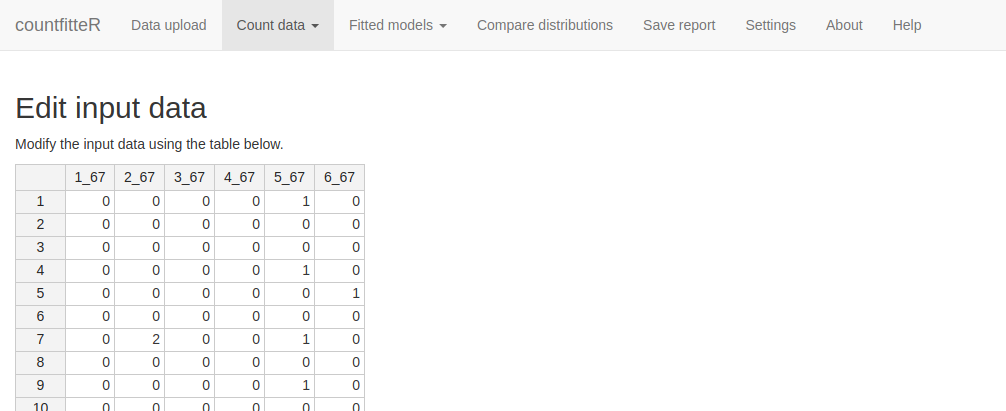
\includegraphics[width=0.99\columnwidth]{fig/cf_cd1.png}
%   \caption{In this section uploaded data can be previewed and modified.}
%     \label{cf_cd1}
% \end{figure}

\begin{figure}[htbp]
  \centering
  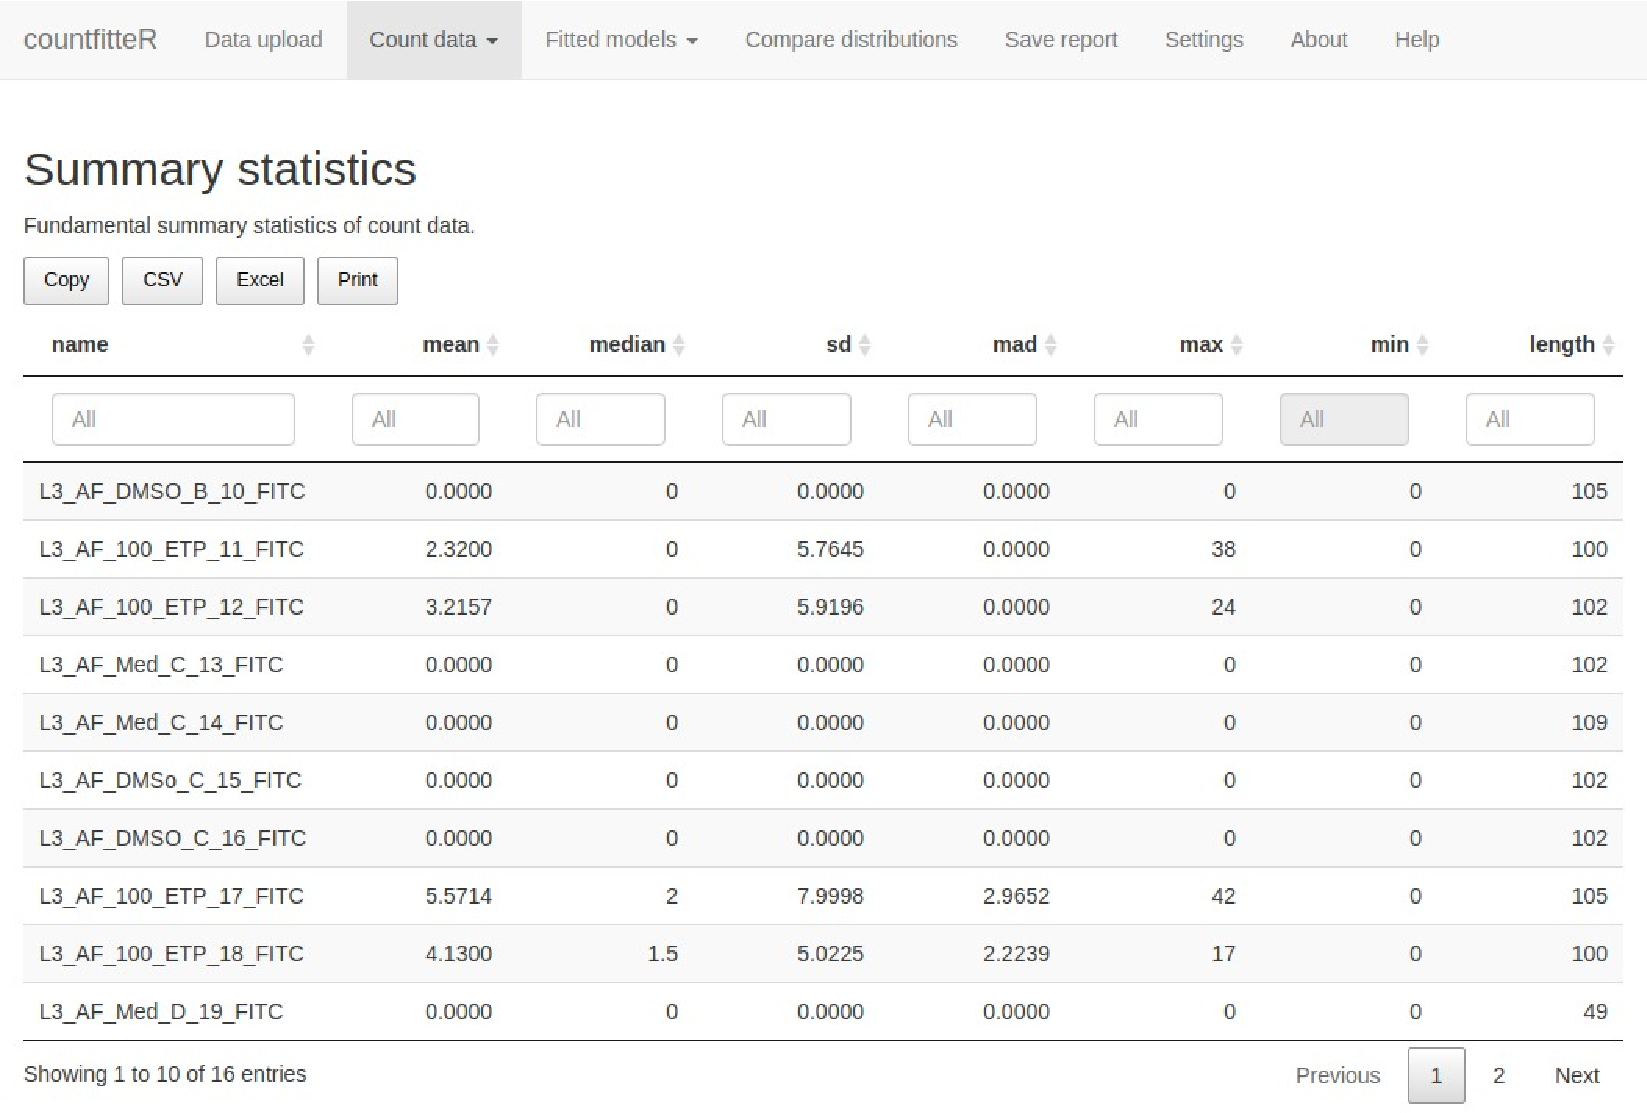
\includegraphics[width=0.99\columnwidth]{fig/cf_cd2.pdf}
  \caption{Interactive table with summary statistics calculated for each count experiment. mean, arithmetic mean of counted foci; median of counted foci; sd, standard deviation of counted foci; max, median absolute deviation of counted foci; min \& max, minimal and maximal number of foci per cell; length, number of counted (analyzed) cells.}
    \label{cf_cd2}
\end{figure}

% \begin{figure}[htbp]
%   \centering
%   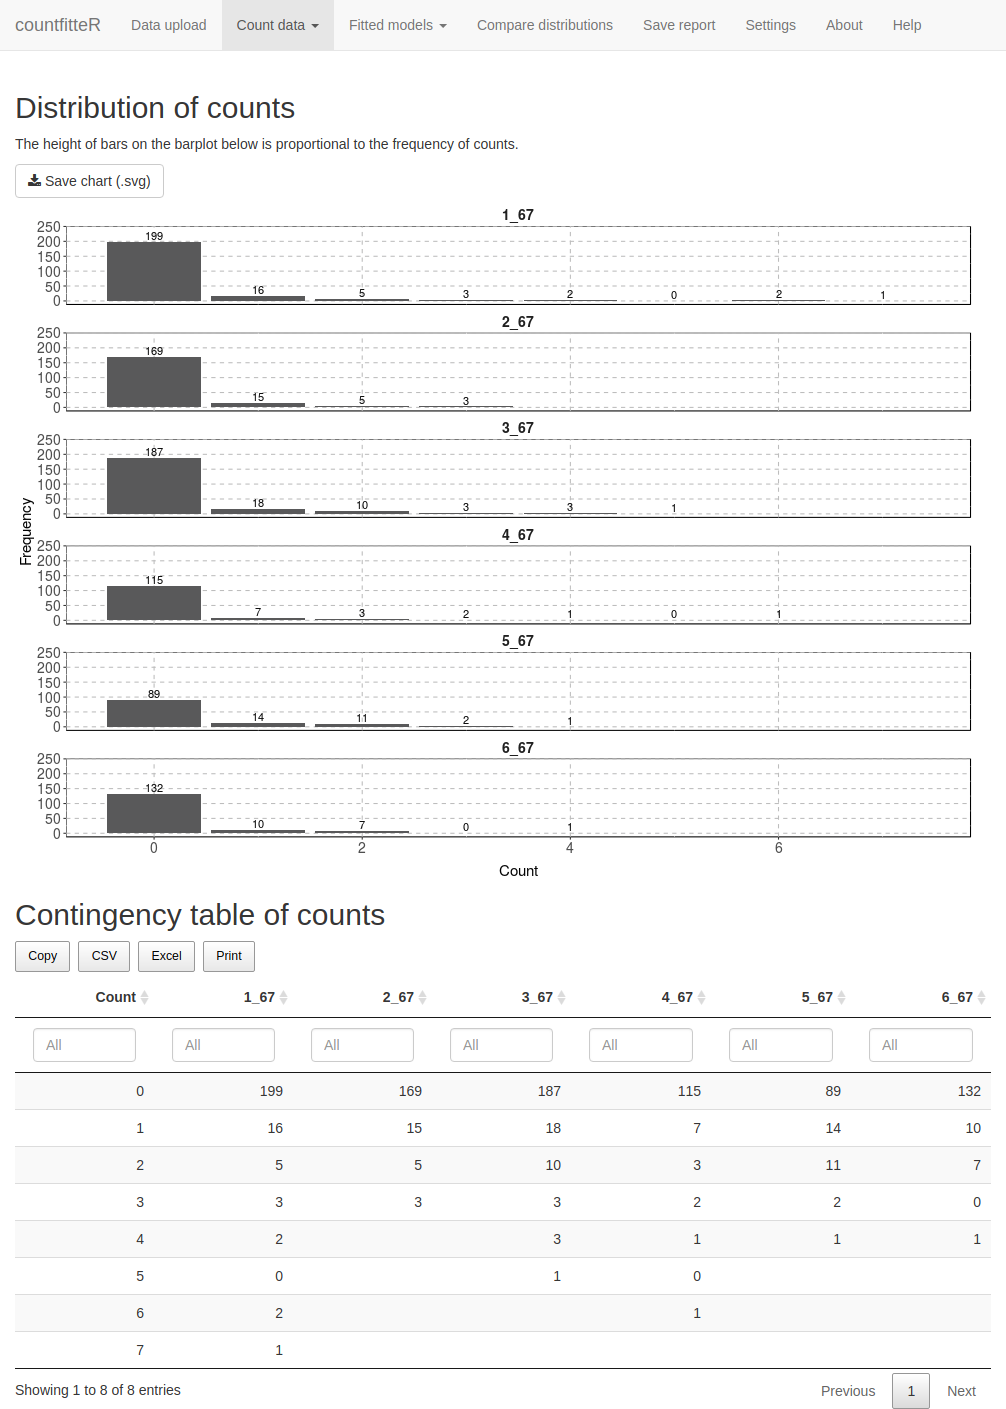
\includegraphics[width=0.99\columnwidth]{fig/cf_cd3.png}
%   \caption{Distribution of counts can be viewed in form of a plot or table.}
%     \label{cf_cd3}
% \end{figure}

Another tab is \textit{Fitted models}. In \textit{Mean value estimate} submenu the mean value estimates and their confidence are displayed on the plots. Below table with summary of estimates, along with the BIC values of their models can be found (Figure \ref{cf_fm1}). The table in \textit{Coefficients} shows estimated coefficients of models
% (Figure \ref{cf_fm2})
. The \emph{countfitteR} selects the most optimal distribution model for each count. Decision can be viewed in the \textit{Decision} submenu (Figure \ref{cf_fm3}).

\begin{figure}[htbp]
  \centering
  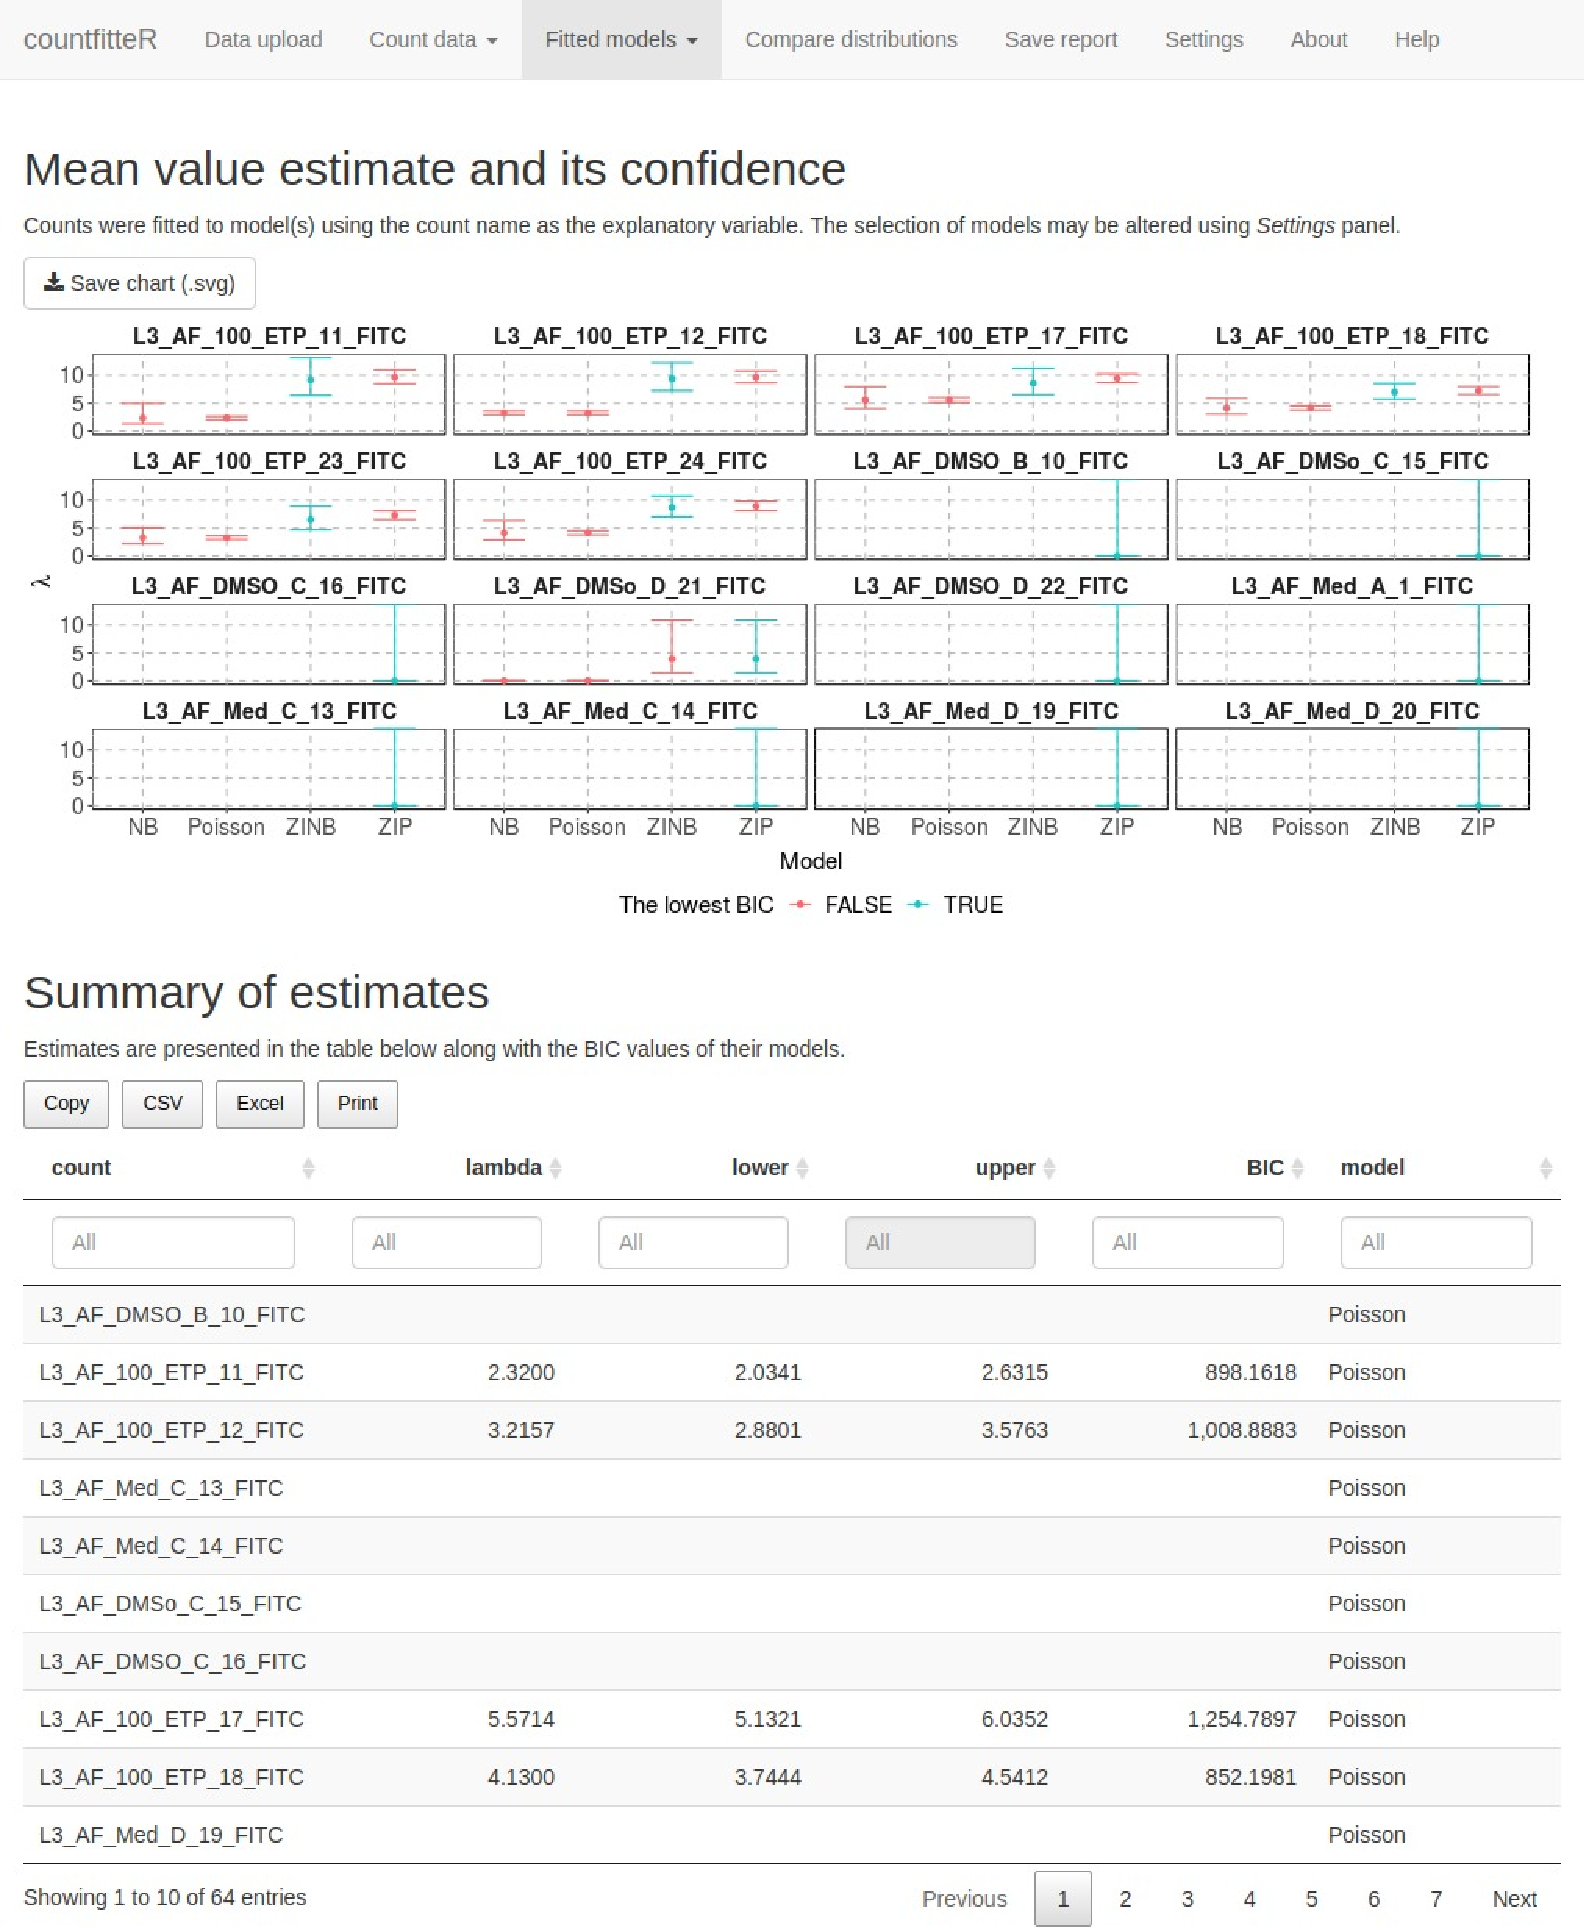
\includegraphics[width=0.99\columnwidth]{fig/cf_fm1.pdf}
  \caption{Plot and a table shows estimated mean value and its confidence.}
    \label{cf_fm1}
\end{figure}

% \begin{figure}[htbp]
%   \centering
%   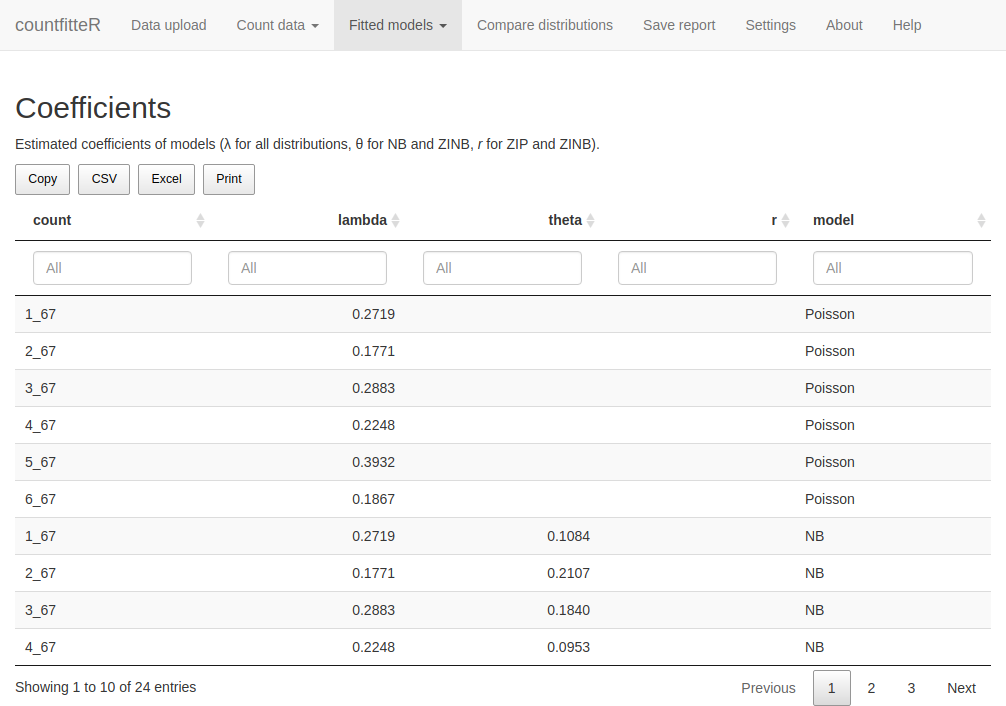
\includegraphics[width=0.99\columnwidth]{fig/cf_fm2.png}
%   \caption{Estimated coefficients values of distribution models.}
%     \label{cf_fm2}
% \end{figure}

\begin{figure}[htbp]
  \centering
  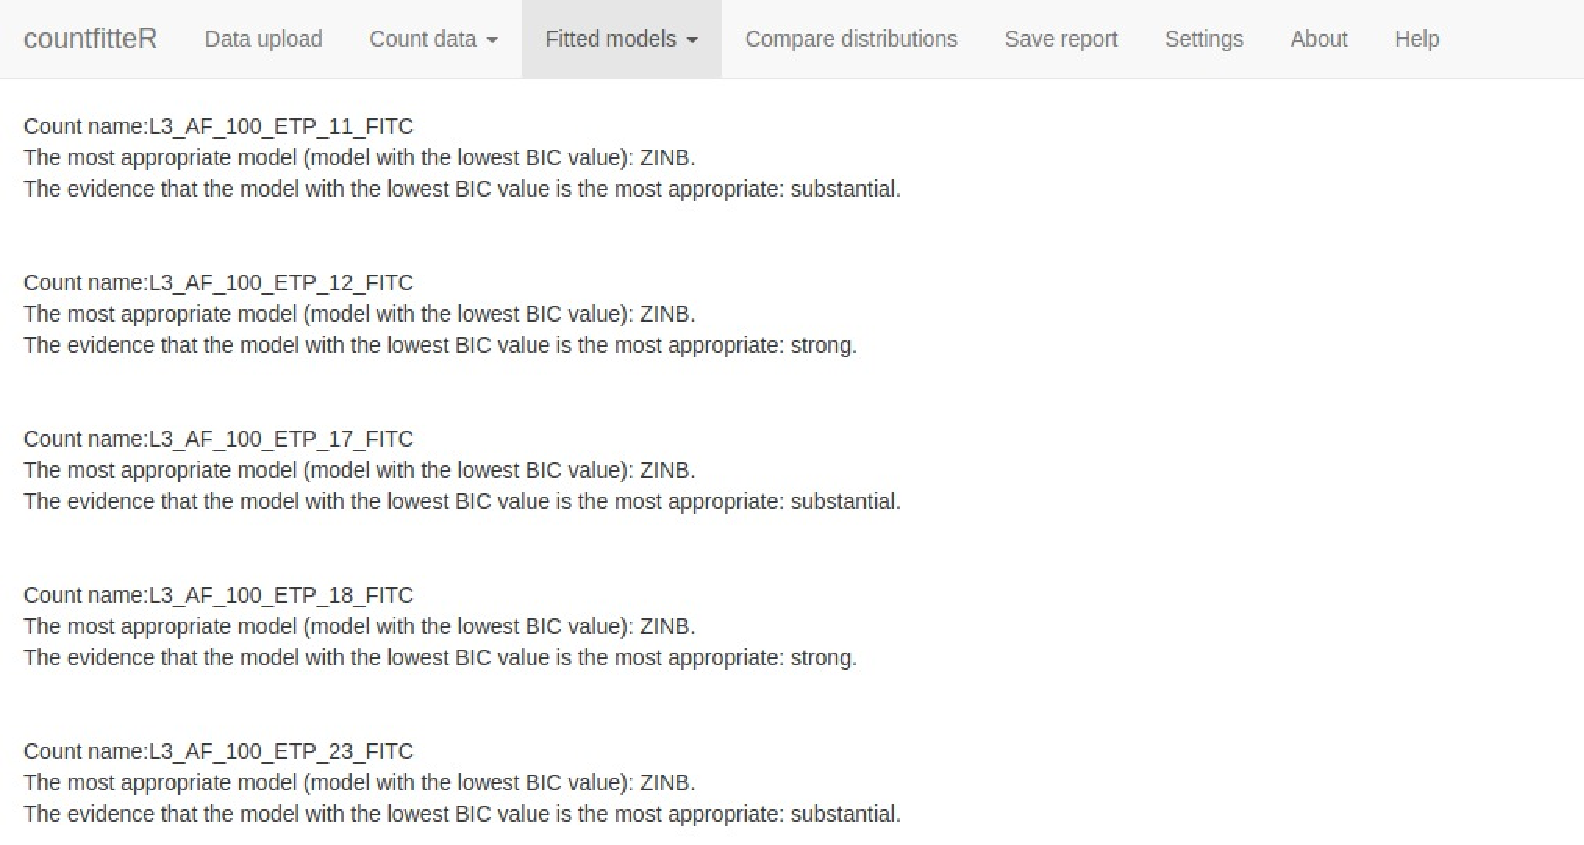
\includegraphics[width=0.99\columnwidth]{fig/cf_fm3.pdf}
  \caption{\emph{countfitteR} decides on the most optimal distribution model.}
    \label{cf_fm3}
\end{figure}

\textit{Compare distributions} tab shows plots with compared empirical distributions of counts, defined by the model fitted to counts. Red points indicate the real number of counts, while bars represents the number of counts estimated by a distribution model (Figure \ref{cf_cmp}).

\begin{figure}[htbp]
  \centering
  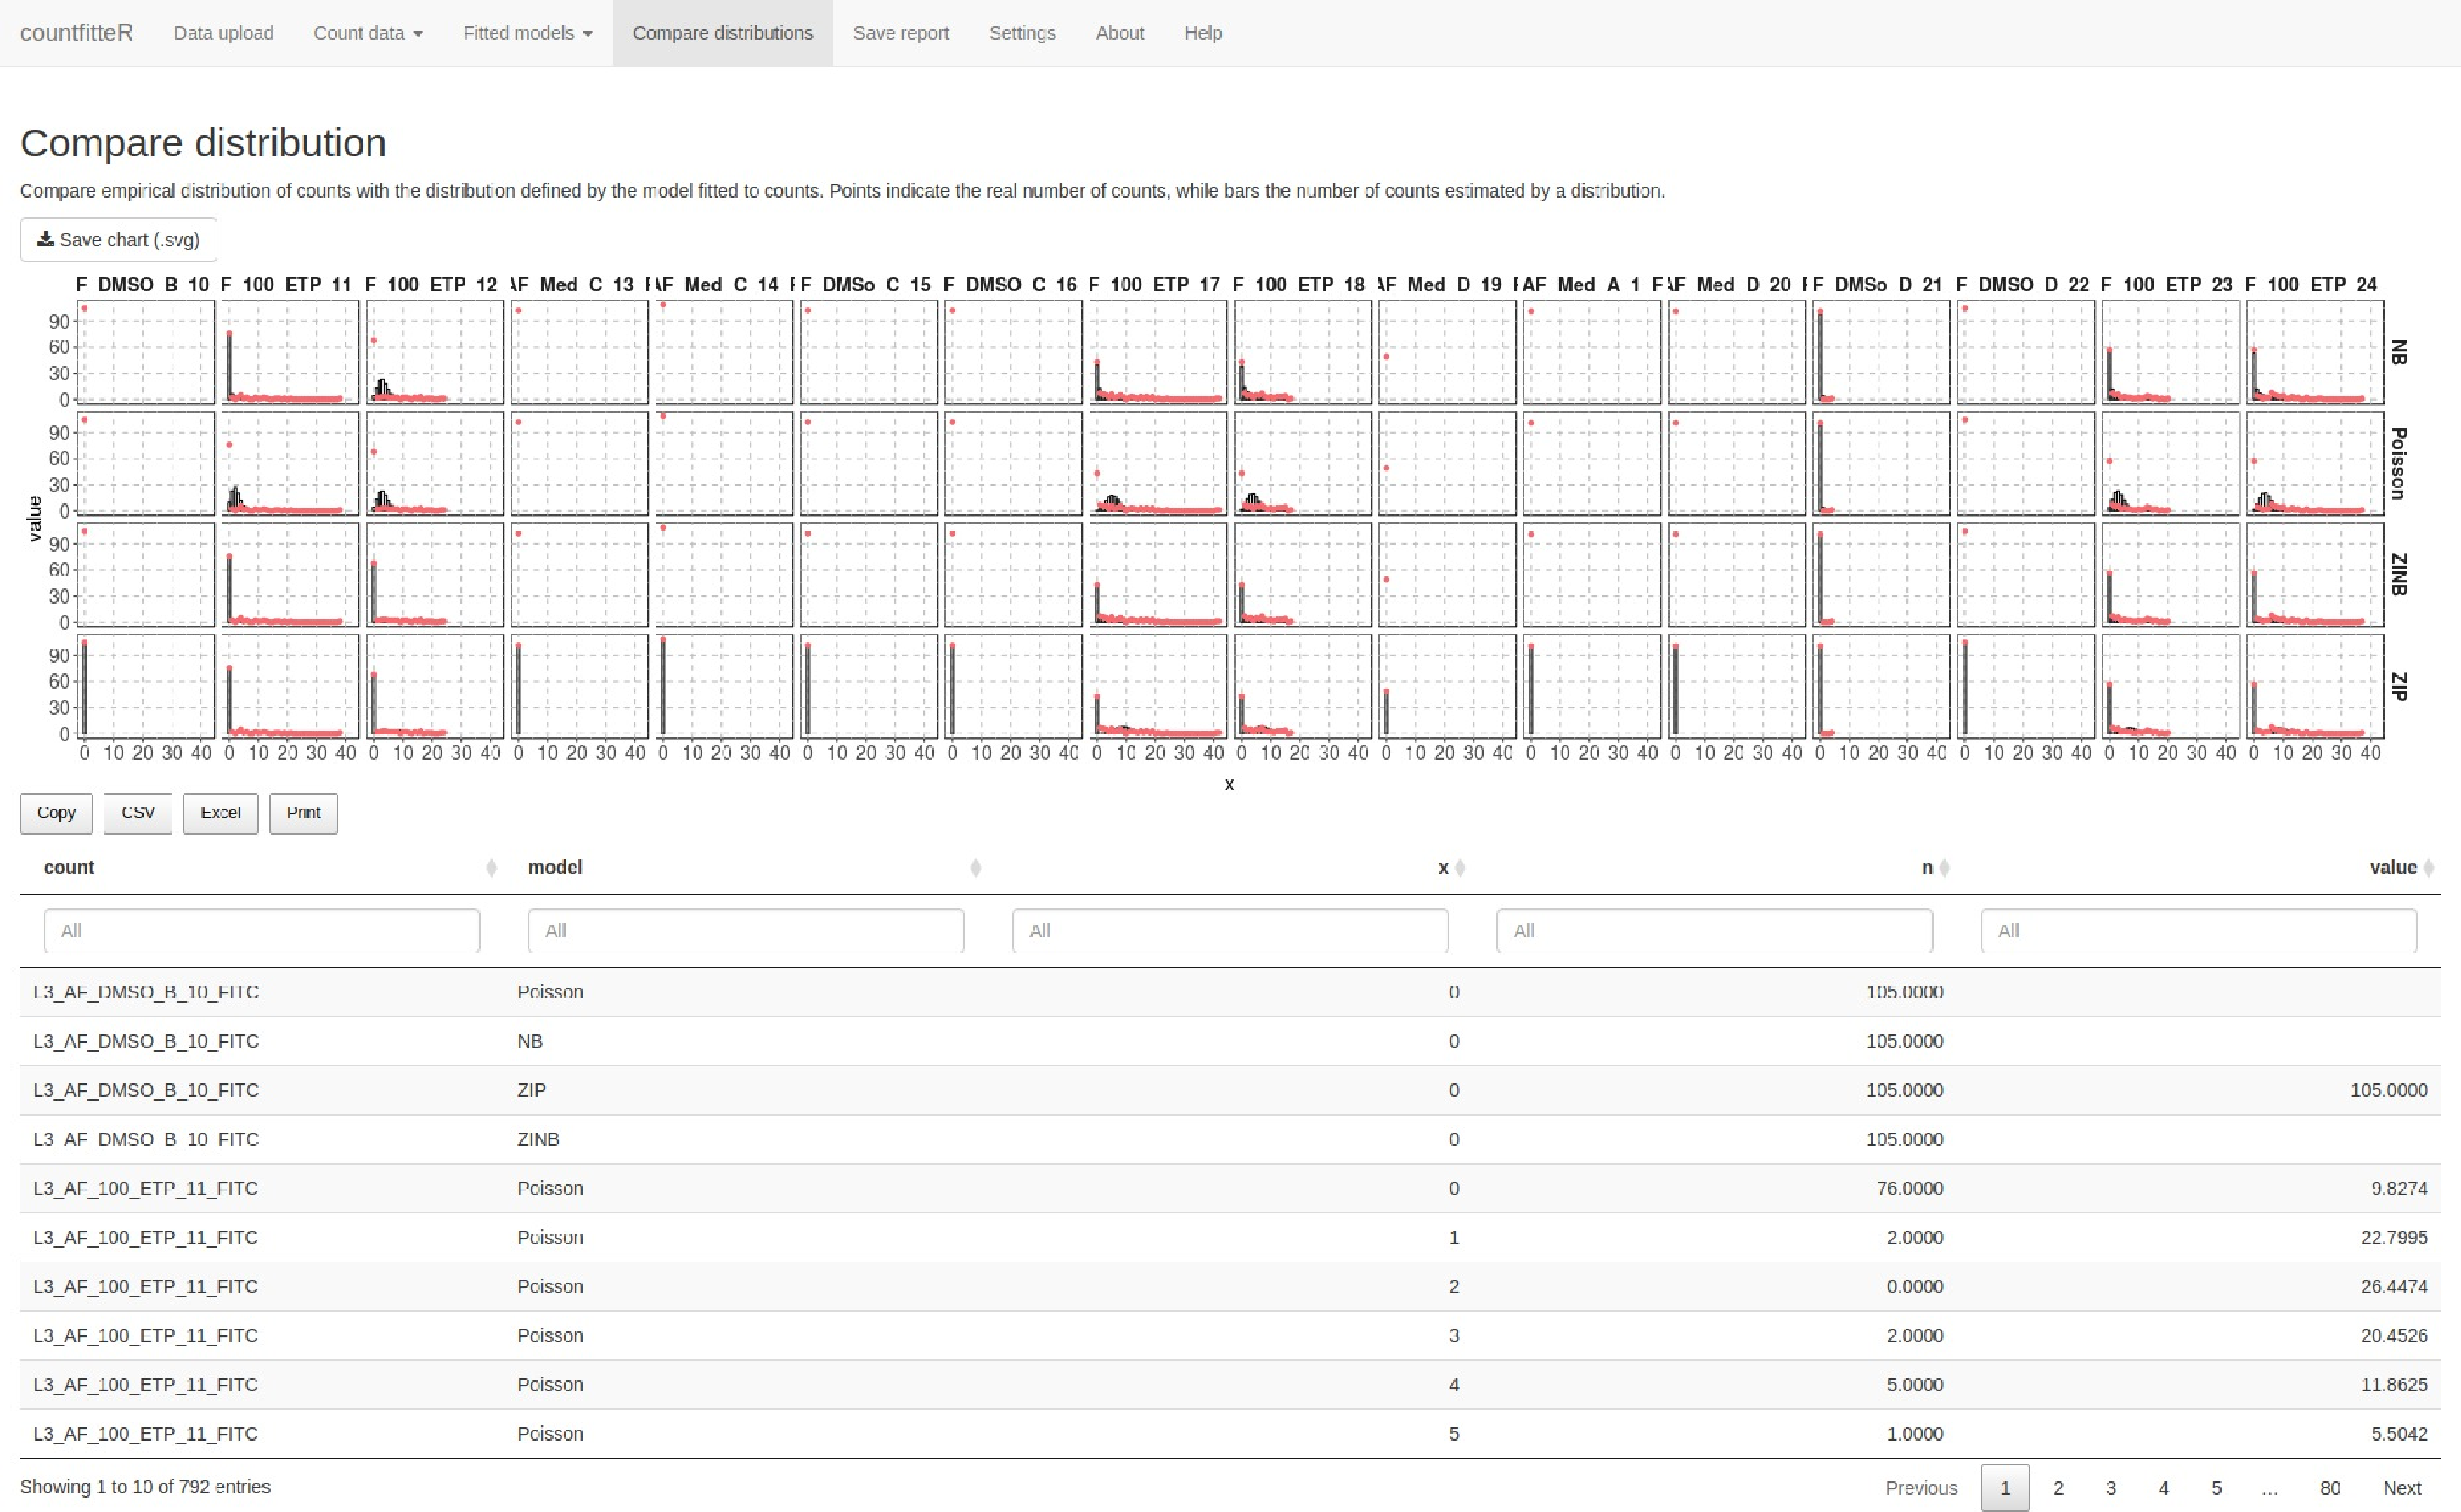
\includegraphics[width=0.99\columnwidth]{fig/cf_cmp.pdf}
  \caption{Comparison of empirical distribution of counts with distribution models.}
    \label{cf_cmp}
\end{figure}

Other tabs are \textit{Save report}, where all the results, obtained from functions described above, can be saved in one file. All reports are properly created only by opening shiny GUI in web browser
% (Figure \ref{cf_rep})
. In \textit{Settings} by default all 4 distribution models are selected for the analyses. The confidence level can be modified. If the \textit{Separate experiment} is marked, it assumes that all counts may come from different distributions
% (Figure \ref{cj_set})
. In \textit{About} tab authors and link to repository of \emph{countfitteR} is found and \textit{Help} there features general tips for each tab. All plots can be saved as Scalable Vector Graphics (SVG) and tables in comma-separated values (CSV) file.

% \begin{figure}[htbp]
%   \centering
%   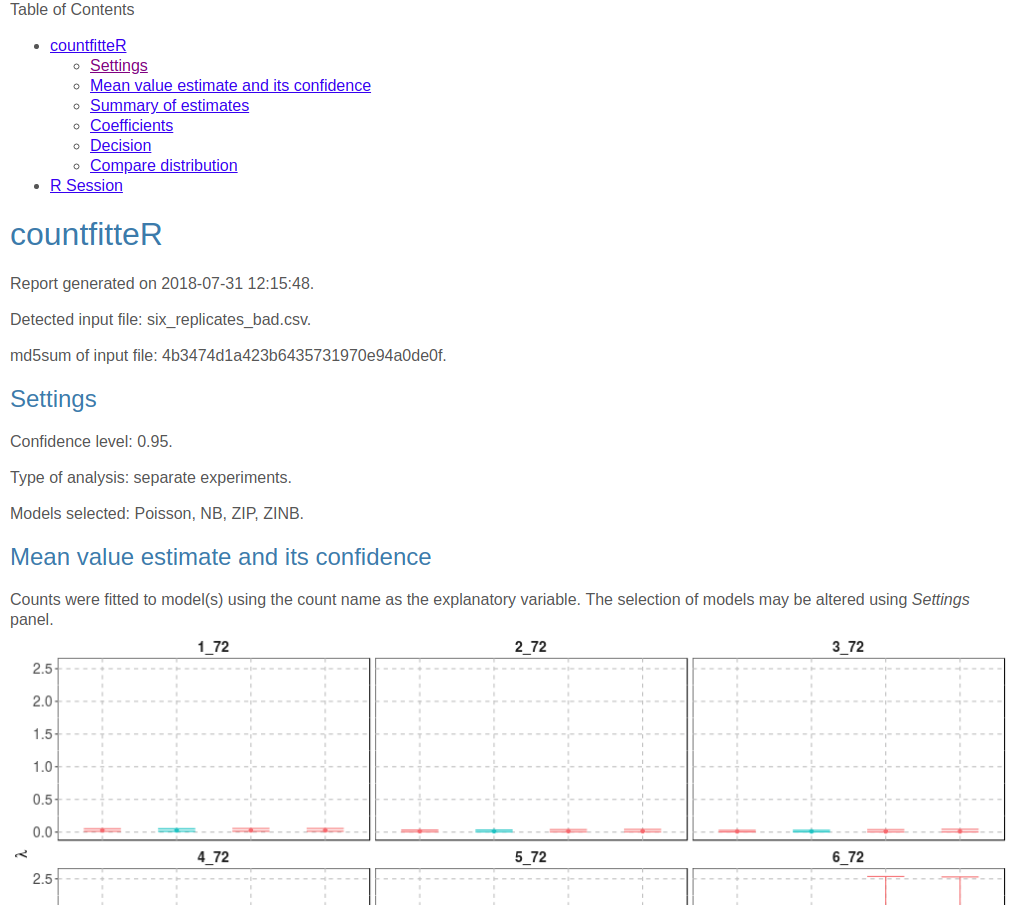
\includegraphics[width=0.99\columnwidth]{fig/cf_rep.png}
%   \caption{Fragment of report generated by \emph{countfitteR}.}
%   \label{cf_rep}
% \end{figure}

% \begin{figure}[htbp]
%   \centering
%   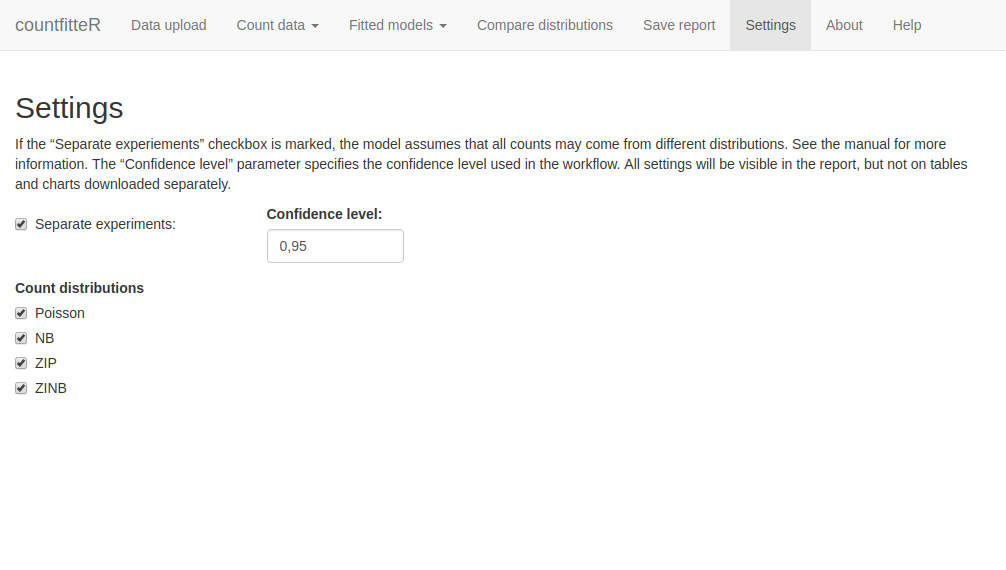
\includegraphics[width=0.99\columnwidth]{fig/cf_set.png}
%   \caption{Options in settings menu.}
%   \label{cj_set}
% \end{figure}

The graphical user interface  (GUI) was created using  the shiny package \citep{shiny}. This allows \emph{countfitteR} to run as a web server, which can be used on a web browser on any personal computer. The software relies on several packages including \emph{ggplot2} \citep{ggplot2}, \emph{MASS} \citep{MASS}, \emph{stats}, \emph{tools} \citep{Rrr}, \emph{shinythemes} \citep{shinythemes}, \emph{rhandsontable} \citep{rhandsontable}, \emph{pscl} \citep{pscl}, \emph{DT} \citep{DT}, \emph{rmarkdown} \citep{rmarkdown}, \emph{reshape2} \citep{reshape2}, \emph{grid} \citep{Rrr}, \emph{gridExtra} \citep{gridextra} and \emph{dplyr}  \citep{dplyr}.


% \begin{figure}[htbp]
%   \centering
%   \includegraphics[width=0.99\columnwidth]{cj_main}
%   \caption{EXAMPLE \emph{countfitteR} shiny app running in the \emph{R Studio} GUI/IDE \citep{}.}
%   \label{figure:cj_m.png}
% \end{figure}
% 
% \begin{figure}[htbp]
%   \centering
%   \includegraphics[width=0.99\columnwidth]{cj_cmp}
%   \caption{EXAMPLE \emph{countfitteR} shiny app running in the \emph{R Studio} GUI/IDE \citep{}.}
%   \label{figure:cj_cmp.png}
% \end{figure}

\section{Functions that can be used from the command line}

\begin{itemize}
    \item \textit{fit\_counts()} - fits counts to distribution models and creates a list of parameters characterizing chosen distribution model.

{\bfseries
\begin{example}
> set.seed(1337)
> df <- data.frame(poisson = rpois(25, 0.3), binomial = rbinom(25, 1, 0.8))
> fc <- fit_counts(df, model = "pois") 
> fc
\end{example}
}


\begin{minipage}{0.45\textwidth}
\begin{example}
$poissonpois
$poissonpois$coefficients
lambda 
  0.48 

$poissonpois$confint
           lower     upper
lambda 0.2570197 0.8049657

$poissonpois$BIC
[1] 50.37931

$poissonpois$model
[1] "pois"

\end{example}
\end{minipage}%
\hfill
\begin{minipage}{0.45\textwidth}
\begin{example}
$binomialpois
$binomialpois$coefficients
lambda 
  0.72 

$binomialpois$confint
           lower    upper
lambda 0.4364839 1.105632

$binomialpois$BIC
[1] 51.04502

$binomialpois$model
[1] "pois"

\end{example}
\end{minipage}

% \end{example}


\item \textit{compare\_fit()} - compares empirical distribution of counts with the distribution defined by the model fitted to counts. Creates data table with distribution values for each unique count.


{\bfseries
\begin{example}
> set.seed(1337)
> df <- data.frame(poisson = rpois(25, 0.3), binomial = rbinom(25, 1, 0.8))
> cmp <- compare_fit(df, fitlist = fit_counts(df, model = "all"))
> cmp
\end{example}
}

\begin{minipage}{0.45\textwidth}
\begin{example}

      count   model x  n     value
1   poisson Poisson 0 17 15.469585
2   poisson Poisson 1  4  7.425401
3   poisson Poisson 2  4  1.782096
4   poisson     ZIP 0 17 16.999975
5   poisson     ZIP 1  4  5.006282
6   poisson     ZIP 2  4  2.188284
7   poisson      NB 0 17 16.511185
8   poisson      NB 1  4  5.959803
9   poisson      NB 2  4  1.814655
10  poisson    ZINB 0 17 17.000111

\end{example}
\end{minipage}%
\hfill
\begin{minipage}{0.45\textwidth}
\begin{example}

      count   model x  n     value
11  poisson    ZINB 1  4  5.006258
12  poisson    ZINB 2  4  2.188188
13 binomial Poisson 0  7 12.168806
14 binomial Poisson 1 18  8.761541
15 binomial     ZIP 0  7 12.168796
16 binomial     ZIP 1 18  8.761519
17 binomial      NB 0  7 12.168873
18 binomial      NB 1 18  8.761455
19 binomial    ZINB 0  7 12.168866
20 binomial    ZINB 1 18  8.761490

\end{example}
\end{minipage}

% \begin{example}
%       count   model x  n     value
% 1   poisson Poisson 0 18 18.894594
% 2   poisson Poisson 1  7  5.290486
% 3   poisson     ZIP 0 18 18.894681
% 4   poisson     ZIP 1  7  5.290388
% ...
% 13 binomial      NB 0  9 13.182392
% 14 binomial      NB 1 16  8.436568
% 15 binomial    ZINB 0  9 13.182335
% 16 binomial    ZINB 1 16  8.436642
% \end{example}

    \item \textit{plot\_fitcmp()} - creates plot from compare\_fit results. The bar charts represent theoretical counts depending on the chosen distribution. Red dots describe the real number of counts.

{\bfseries
\begin{example}
> set.seed(1337)
> df <- data.frame(poisson = rpois(25, 0.3), binomial = rbinom(25, 1, 0.8))
> cmp <- compare_fit(df, fitlist = fit_counts(df, model = "all"))
> plot_fitcmp(cmp)
\end{example}
}

\begin{figure}[htbp]
  \centering
  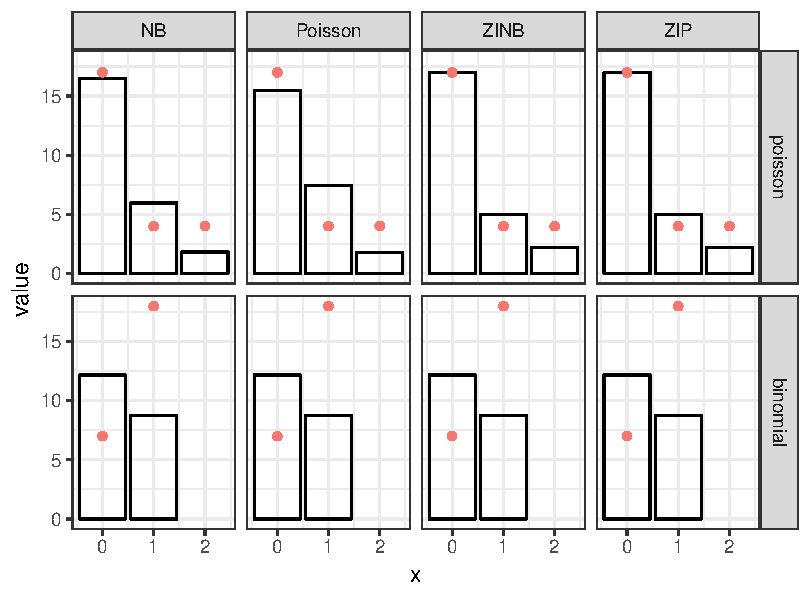
\includegraphics[width=0.99\columnwidth]{fig/Rplot1.pdf}
  \label{figure:Rplot.png}
\end{figure}

\item \textit{summary\_fitlist()} - creates data frame from a list created by \textit{fit\_counts()} function with additional attributes. Data frame with summarised results of all distribution models.

{\bfseries
\begin{example}
> set.seed(1337)
> df <- data.frame(poisson = rpois(25, 0.3), binomial = rbinom(25, 1, 0.8))
> fc <- fit_counts(df, model = "all")
> summary_fitlist(fc) 
\end{example}
}
% \footnotesize
{\scriptsize
\begin{example}
                 count    lambda     lower     upper      BIC        theta            r   model
poisson_pois   poisson 0.4800000 0.2570197 0.8049657 50.37931           NA           NA Poisson
binomial_pois binomial 0.7200000 0.4364839 1.1056323 51.04502           NA           NA Poisson
poisson_zip    poisson 0.8742154 0.3466865 2.2044485 51.90185           NA 4.509350e-01     ZIP
binomial_zip  binomial 0.7200058 0.4536344 1.1427889 54.26400           NA 4.691600e-06     ZIP
poisson_nb     poisson 0.4800000 0.2395727 0.8946153 52.99679 1.455411e+00           NA      NB
binomial_nb   binomial 0.7200000 0.4364790 1.1056475 54.26417 4.703206e+04           NA      NB
poisson_zinb   poisson 0.8741759 0.3466513 2.2044732 55.12084 2.104895e+04 4.509217e-01    ZINB
binomial_zinb binomial 0.7200000 0.4536297 1.1427824 57.48291 1.839077e+05 3.316485e-06    ZINB
\end{example}
}

\item \textit{dZIP()} - generates density value for the zero inflated Poisson distribution.

{\bfseries
\begin{example}
> set.seed(1337)
> dZIP(10, 2, 0.6)
\end{example}
}
\begin{example}
[1] 2.291391e-05
\end{example}


\item \textit{rZIP()} - generates random quantiles for the zero inflated Poisson distribution.

{\bfseries
\begin{example}
> set.seed(1337)
> rZIP(10, 2, 0.6) 
\end{example}
}
\begin{example}
[1] 0 3 0 0 3 1 0 2 2 2
\end{example}


\item \textit{rZINB} - generates density value for the zero-inflated negative binomial distribution.

{\bfseries
\begin{example}
> set.seed(1337)
> dZINB(seq(1:5), 5, 5, 0.6)
\end{example}
}
\begin{example}
[1] 0.04687500 0.07031250 0.08203125 0.08203125 0.07382813
\end{example}


\item \textit{dZINB()} - generates random quantiles for the zero-inflated negative binomial distribution.

{\bfseries
\begin{example}
> set.seed(1337)
> rZIP(10, 2, 0.6) 
\end{example}
}
\begin{example}
[1] 0 0 1 0 3 0 0 1 2 0
\end{example}

\end{itemize}
% fitCounts \\
% Estimates are presented in the table below along with the BIC values of their models.
% Function is used to estimate the best distribution models for given data
% Fit count is used to fit counts to different distribution models.
% function is used to create a list of parameters characterizing chosen model. Those attributes are: 
% \begin{itemize}
%     \item lambda - Poisson parameter (average number of foci per cell). the estimated value of mean
%     \item confint - lambda confidence intervals
%     \item BIC - Bayesian Criterion Information, important criterion for model selection
%     \item model - information of applied model
% \end{itemize}
% 
% summaryFitlist \\
% summary fitlist creates data frame from a list created by fit counts function with additional attributes as:
% \begin{itemize}
%     \item theta - dispersion parameter.
%     \item r - zero inflation (fraction of cells treated by system as having no foci regardless of their real state).
% \end{itemize}
% Estimated coefficients of models (lambda for all distributions, theta for NB and ZINB, r for ZIP and ZINB).
% 
% compareFit and plotFitcmp \\
% compare fit function compares empirical distribution of counts with the distribution defined by the model fitted to counts. 
% plot fitcmp creates plot from compare fit results. 
% Points indicate the real number of counts, while bars the number of counts estimated by a distribution.


\section{Results and conclusion.}

This article describes the \emph{countfitteR} package. The package is designed for the analysis of count data. Simultaneously it uses four distribution models for determination of the most optimal one for the given count data set based on an objective statistical measure.

When analyzing the count data, it is important to select the appropriate distribution model. For example, in our use case, we start from a single cell population that has been exposed to different conditions (sill vs. cryo-preservation). All further steps (incl. immunohistochemical staining, storage, measurement) are identical. At first glance, one may assume that the measured values of both conditions have the same distribution. This assessment is incumbent on the domain knowledge of the respective scientist. The scientist must decide whether the measured data display a Poisson distribution, for example. For example, \citet{deagle_quantification_2006} assumed a random Poisson process to model quantitative estimates of DNA damage of highly degraded DNA from faeces samples. However, it is not recommended to assume that all measurement data of an experiment have the same distribution. There is empirical support that this assumption is not correct \citep{myung_counting_2000}. Reading the literature for the analysis of DNA double-strand breaks, many authors assume a Poisson distribution. A justification for this decision usually is not given. Rather, one should assume that the samples have different distribution models. In such cases the term separated distributions is used. 

The \emph{countfitteR} software addresses this problem by supporting the user in selecting a more suitable model. A limitation of the approach is the number of models tested. Currently, four models are being tested that are suitable for counting data. These are models that are generally described in the literature for numerical data. \emph{countfitteR} can, however, select these from objective criteria and thus support decision making. There is a consent to use a information criterion such as the Bayes information criterion (BIC) \citep{myung_counting_2000, zucchini_introduction_2000}. From a pragmatic point of view this is a progress compared to existing approaches. We see the specification of the model and the justification for the choice of model as an important approach for reproducible research.

One of the most important characteristics of \emph{countfitteR} and its shiny GUI is the ability to  decide which distribution is optimal for the given dataset. The shiny web server is easy to use by researchers who do not have experience using command line, in statistics and bioinformatics. One limitation of the software is the fixed number ($n = 1$) of parameters that can be analyzed via the GUI. As reviewed by us \citep{ruhe_molecular_2019} there are further \textit{countable} biomarkers described in the scientific literature and clinical trials. However, the integration of multiple simultaneous analysis is currently not planned since such tasks presumably are better handled via dedicated programmatic approaches.
Currently one can find distribution analysis software like \emph{ShrinkBayes} \citep{shrinkbayes}, \emph{COUNT} \citep{COUNT}, \emph{pscl} \citep{pscl}, \emph{countreg} \citep{countreg} and \emph{CountsEPPM} \citep{countseppm} that analyses distributions of count datasets but none of them have user friendly interface. All of the listed packages must be run from the command line. 
Listed software is limited and focuses on a specific kind of data (e.g. sequencing) or uses only one distribution model (e.g. either Poisson or binomial). \emph{countfitteR} however looks simultaneously at four different distribution models to asses the most optimal one. It is also not restricted to only one type of data. 
%Moreover, unlike \emph{countfitteR}, they do not have functions that compare distributions and decides the most optimal one.

For reproducible research, the availability of algorithmic tools for accessing and analyzing open data collections is of great benefit \cite{lahti_retrieval_2017}. Reproducible means that a detailed description of research workflow allows other users to replicate published results precisely \citep{leeper_archiving_2014}. The code is explained and the most important functions are detailed \citep{thioulouse_online_2010}. 
Used hardware, wetware and software also needs to be listed to master a workflow as a minor change may lead to a different result \citep{rodiger_r_2015}. 
All this steps are necessary for other researchers to reproduce the results and those results that are not reproducible are generally considered invalid by the scientific community \citep{rodiger_r_2015}.
%as the scientific misconduct and fraud have shaken the scientific community on several occasions \citep{rodiger_r_2015}.
There are some packages like \emph{rctrack} \citep{liu_r_2014} and \emph{archivist} \citep{Biecek_2017} that automatically archive data files, code files, and other details. They are also creating new ways to retrieve and validate previously calculated R objects. 

Since \emph{countfitteR} is based on R, it can make use of various tools for reproducible research. In our case this is achieved through generating an \emph{rmarkdown} \citep{rmarkdown} report file using the shiny GUI. The report contains the date of generation, name of uploaded file, the md5 hash value and information describing working environment. This includes R version, platform, operating system and its version, list of all packages and attached ones. 

The package is written in accordance with modern standards described in \cite{R_Packages}. We have implemented \emph{testthat} \citep{testthat} to ensure that all functions in \emph{countfitter} work according to their \textit{expectation}. We are also using \emph{Travis CI} (\url{https://travis-ci.org/}) for build testings and \emph{shinytest} \citep{shinytest} to be sure that shiny GUI works as expected by the developers.

%At the beginning of the report there is the date of generation, below is the name of detected uploaded file and its md5sum. At the very end of document there is an information about used environment. This includes R version, platform, operating system and its version, list of all packages and attached ones.

% \citep{leeper_archiving_2014,thioulouse_online_2010,rodiger_r_2015,liu_r_2014,Biecek_2017}

Most of the functions in \emph{countfitteR} are available as shiny server, that can run on local pc. It can be applied in the analysis of any type of count data. The most important functions of the package can be accessed from command line, integration into other analysis pipelines.

\section{Acknowledgments}

We want to thank Madeleine Ruhe for $\gamma$H2AX data.

\bibliography{Chilmoniuk}

\address{Jaros\l{}aw Chilimoniuk\\
  University of Wroc\l{}aw\\
  Pl. Uniwersytecki 1, Wroc\l{}aw\\
  Poland\\
  ORCiD: 0000-0001-5467-018X\\
  \email{jaroslaw.chilimoniuk@gmail.com}}

\address{Alicja Gosiewska\\
  Warsaw University of Technology\\
  Pl. Politechniki 1, Warszawa\\
  Poland\\
  ORCiD: 0000-0001-8926-582X\\
  \email{alicjagosiewska@gmail.com}}


\address{Stefan R\"{o}diger (corresponding author)\\
  Brandenburg University of Technology Cottbus - Senftenberg\\
  Universit\"atsplatz 1, Senftenberg\\
  Germany\\
  ORCiD: 0000-0002-1441-6512\\
  \email{stefan.roediger@b-tu.de}}

\address{Micha\l{} Burdukiewicz (corresponding author)\\
  Warsaw University of Technology\\
  Pl. Politechniki 1, Warszawa\\
  Poland\\
  ORCiD: 0000-0001-8926-582X\\
  \email{michalburdukiewicz@gmail.com}}
